\documentclass[tikz,border=8pt]{standalone}
\usepackage[utf8]{inputenc}
\usepackage{lmodern}
\usepackage[T1]{fontenc}
\usepackage{amsmath,amssymb}
\usetikzlibrary{shapes.geometric, arrows.meta, positioning, calc}

\begin{document}
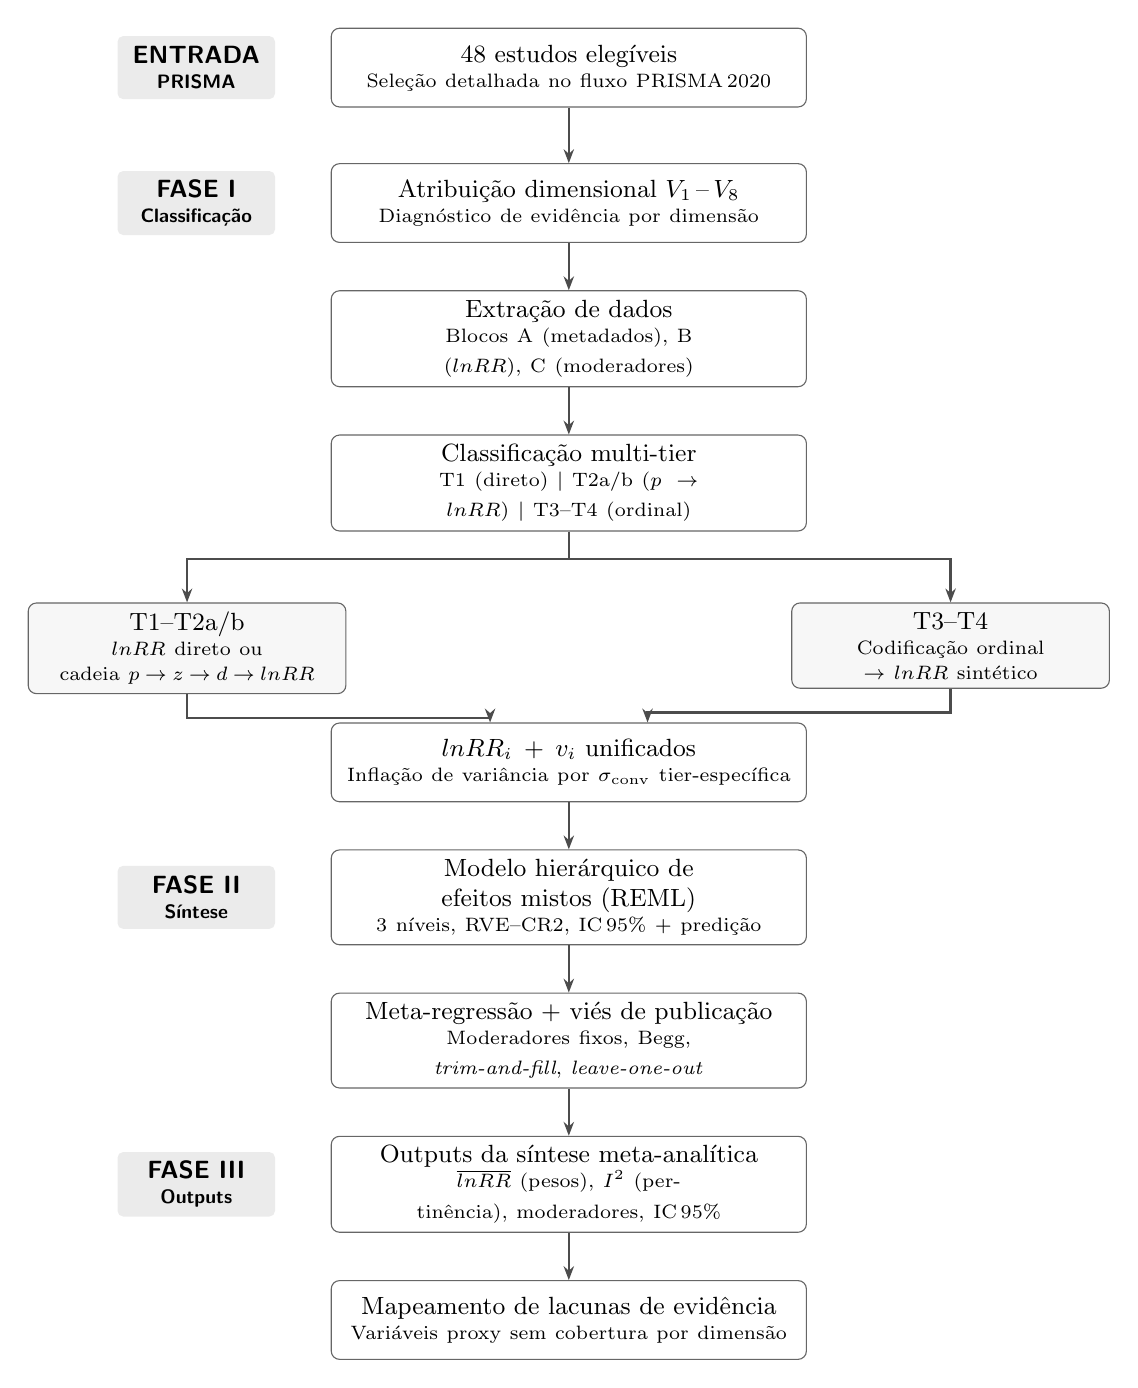
\begin{tikzpicture}[
  phase/.style={
    fill=black!8, draw=none,
    font=\sffamily\bfseries\small,
    minimum width=2.0cm, minimum height=0.8cm,
    align=center, rounded corners=2pt
  },
  mainbox/.style={
    draw=black!60, fill=white,
    font=\small, align=center,
    minimum width=6.0cm, minimum height=1.0cm,
    rounded corners=3pt, text width=5.8cm
  },
  branchbox/.style={
    draw=black!60, fill=black!3,
    font=\small, align=center,
    minimum width=4.0cm, minimum height=0.9cm,
    rounded corners=3pt, text width=3.8cm
  },
  sidebox/.style={
    draw=black!40, dashed, fill=yellow!6,
    font=\small, align=center,
    minimum width=4.2cm, minimum height=0.9cm,
    rounded corners=3pt, text width=4.0cm
  },
  arr/.style={-{Stealth[length=5pt]}, thick, black!70},
  darr/.style={-{Stealth[length=4pt]}, thin, black!40, dashed},
  node distance=0.6cm
]

%% ENTRADA: 48 estudos do PRISMA
\node[phase] (ph1) {ENTRADA\\[-2pt]{\scriptsize PRISMA}};

\node[mainbox, right=0.7cm of ph1] (input48)
  {48 estudos elegíveis\\[-2pt]
   {\scriptsize Seleção detalhada no fluxo PRISMA\,2020}};

%% NOS removida do artigo — caixa eliminada

%% FASE I — Classificação
\node[phase] at (ph1 |- input48.south) [below=0.8cm] (ph3)
  {FASE I\\[-2pt]{\scriptsize Classificação}};

\node[mainbox, right=0.7cm of ph3] (dim)
  {Atribuição dimensional $V_1$\,--\,$V_8$\\[-2pt]
   {\scriptsize Diagnóstico de evidência por dimensão}};
\draw[arr] (input48) -- (dim);

\node[mainbox, below=of dim] (ext)
  {Extração de dados\\[-2pt]
   {\scriptsize Blocos A (metadados), B ($lnRR$), C (moderadores)}};
\draw[arr] (dim) -- (ext);

\node[mainbox, below=of ext] (tier)
  {Classificação multi-tier\\[-2pt]
   {\scriptsize T1 (direto) $\mid$ T2a/b ($p \!\rightarrow\! lnRR$) $\mid$ T3--T4 (ordinal)}};
\draw[arr] (ext) -- (tier);

%% Ramificacao T1-T2 vs T3-T4
\node[branchbox, below left=0.9cm and -0.2cm of tier] (t12)
  {T1--T2a/b\\[-2pt]
   {\scriptsize $lnRR$ direto ou}\\[-2pt]
   {\scriptsize cadeia $p\!\rightarrow\!z\!\rightarrow\!d\!\rightarrow\!lnRR$}};

\node[branchbox, below right=0.9cm and -0.2cm of tier] (t34)
  {T3--T4\\[-2pt]
   {\scriptsize Codificação ordinal}\\[-2pt]
   {\scriptsize $\rightarrow$ $lnRR$ sintético}};

\draw[arr] (tier.south) -- ++(0,-0.35) -| (t12.north);
\draw[arr] (tier.south) -- ++(0,-0.35) -| (t34.north);

%% Convergencia
\coordinate (midconv) at ($(t12.south)!0.5!(t34.south) + (0,-0.9)$);

\node[mainbox] at (midconv) (conv)
  {$lnRR_i + v_i$ unificados\\[-2pt]
   {\scriptsize Inflação de variância por $\sigma_{\mathrm{conv}}$ tier-específica}};

\draw[arr] (t12.south) -- ++(0,-0.3) -| ([xshift=-1.0cm]conv.north);
\draw[arr] (t34.south) -- ++(0,-0.3) -| ([xshift=1.0cm]conv.north);

%% MICE impratic\'{a}vel (94\% sem dados completos) — caixa eliminada

%% FASE II
\node[phase] at (ph3 |- conv.south) [below=0.8cm] (ph4)
  {FASE II\\[-2pt]{\scriptsize Síntese}};

\node[mainbox, right=0.7cm of ph4] (model)
  {Modelo hierárquico de efeitos mistos (REML)\\[-2pt]
   {\scriptsize 3 níveis, RVE--CR2, IC\,95\% + predição}};
\draw[arr] (conv) -- (model);

\node[mainbox, below=of model] (metareg)
  {Meta-regressão + viés de publicação\\[-2pt]
   {\scriptsize Moderadores fixos, Begg, \textit{trim-and-fill}, \textit{leave-one-out}}};
\draw[arr] (model) -- (metareg);

%% FASE III
\node[phase] at (ph4 |- metareg.south) [below=0.8cm] (ph5)
  {FASE III\\[-2pt]{\scriptsize Outputs}};

\node[mainbox, right=0.7cm of ph5] (out)
  {Outputs da síntese meta-analítica\\[-2pt]
   {\scriptsize $\overline{lnRR}$ (pesos), $I^2$ (pertinência), moderadores, IC\,95\%}};
\draw[arr] (metareg) -- (out);

\node[mainbox, below=of out] (gaps)
  {Mapeamento de lacunas de evidência\\[-2pt]
   {\scriptsize Variáveis proxy sem cobertura por dimensão}};
\draw[arr] (out) -- (gaps);

\end{tikzpicture}
\end{document}
